\documentclass{report} 

\usepackage{graphicx}

\begin{document}  

%============================%
%                            %
%   Cholesky factorization   %
%                            %
%============================%
\section{Cholesky factorization}

%----------------%
%    Cholesky    %
%----------------%
\begin{figure}[ht]
  \centering
  \setlength{\unitlength}{1mm}
  \begin{picture}(60,60)(0,0)
%-> \thicklines\put(0,0){\framebox(63,80){}}
    \put( 1,0){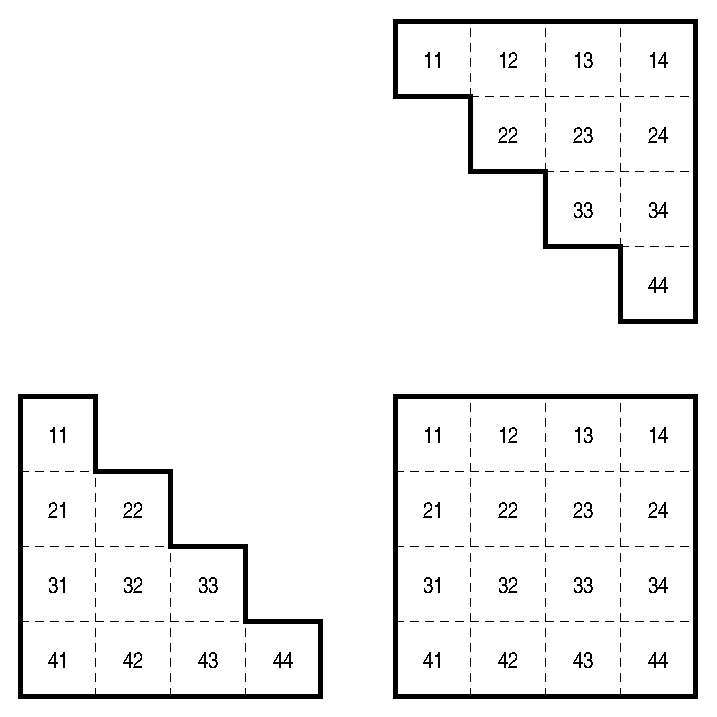
\includegraphics[height=6.0cm]{Cholesky.eps}}
  \end{picture}
\end{figure}

\begin{equation}
  \begin{array}{ll}
    \mbox{Row 1}         & \mbox{Row 2}                         \\
    a_{11} = l_{11}^2      & a_{22} = l_{12}^2      + l_{22}^2      \\
    a_{12} = l_{12} l_{11} & a_{23} = l_{12} l_{13} + l_{22} l_{23} \\
    a_{13} = l_{13} l_{11} & a_{24} = l_{12} l_{14} + l_{22} l_{24} \\
    a_{14} = l_{14} l_{11} &                                        \\ 
                           &                                        \\
    \mbox{Row 3}                                         & \; \mbox{Row 4}                                    \\
    a_{33} = l_{13}^2 + l_{23}^2 + l_{33}^2                & \; a_{44} = l_{14}^2 + l_{24}^2 + l_{34}^2 + l_{44}^2 \\
    a_{34} = l_{13} l_{14} + l_{23} l_{24} + l_{33} l_{34} & \; 
  \end{array}
\end{equation}

\begin{equation}
  \begin{array}{ll}
    \mbox{Row 1}           & \mbox{Row 2}                           \\
    l_{11} = \sqrt{a_{11}^2} & l_{22} = \sqrt{a_{22} - l_{12}^2}        \\
    l_{12} = a_{12} / l_{11} & l_{23} = (a_{23} - l_{12} l_{13})/l_{22} \\
    l_{13} = a_{13} / l_{11} & l_{24} = (a_{24} - l_{12} l_{14})/l_{22} \\
    l_{14} = a_{14} / l_{11} &                                          \\ 
                             &                                          \\
    \mbox{Row 3}                                           & \; \mbox{Row 4}                                          \\
    l_{33} = \sqrt{a_{33} - l_{13}^2 + l_{23}^2}             & \; l_{44} = \sqrt{a_{44} - l_{14}^2 - l_{24}^2 - l_{34}^2} \\
    l_{34} = (a_{34} - l_{13} l_{14} - l_{23} l_{24})/l_{33} & \; 
  \end{array}
\end{equation}

\clearpage

%=======================================%
%                                       %
%   Incomplete Cholesky factorization   %
%                                       %
%=======================================%
\section{Incomplete Cholesky factorization}

%-----------------------%
%  Incomplete Cholesky  %
%-----------------------%
\begin{figure}[ht]
  \centering
  \setlength{\unitlength}{1mm}
  \begin{picture}(60,60)(0,0)
%-> \thicklines\put(0,0){\framebox(63,80){}}
    \put( 1,0){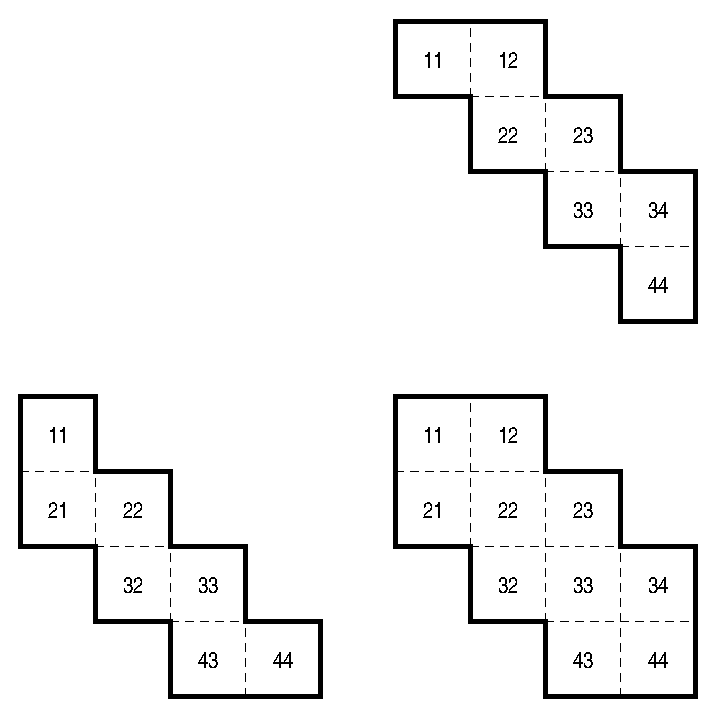
\includegraphics[height=6.0cm]{Incomplete_Cholesky.eps}}
  \end{picture}
\end{figure}

\begin{equation}
  \begin{array}{ll}
    \mbox{Row 1}         & \mbox{Row 2}                             \\
    a_{11} = l_{11}^2      & a_{22} = l_{12}^2      + l_{22}^2      \\
    a_{12} = l_{12} l_{11} & a_{23} = l_{22} l_{23}                 \\
    a_{13} = 0             & a_{24} = 0                             \\
    a_{14} = 0             &                                        \\ 
                           &                                        \\
    \mbox{Row 3}               & \; \mbox{Row 4}                    \\
    a_{33} = l_{23}^2 + l_{33}^2 & \; a_{44} = l_{34}^2 + l_{44}^2  \\
    a_{34} = l_{33} l_{34}       & \; 
  \end{array}
\end{equation}

\begin{equation}
  \begin{array}{ll}
    \mbox{Row 1}           & \mbox{Row 2}                        \\
    l_{11} = \sqrt{a_{11}^2} & l_{22} = \sqrt{a_{22} - l_{12}^2} \\
    l_{12} = a_{12} / l_{11} & l_{23} = a_{23}/l_{22}            \\
    l_{13} = 0               & l_{24} = 0                        \\
    l_{14} = 0               &                                   \\ 
                             &                                   \\
    \mbox{Row 3}                      & \; \mbox{Row 4}                      \\
    l_{33} = \sqrt{a_{33} - l_{23}^2} & \; l_{44} = \sqrt{a_{44} - l_{34}^2} \\
    l_{34} = a_{34}/l_{33}            & \; 
  \end{array}
\end{equation}

\clearpage

%================================================%
%                                                %
%   General cartesian system, compass notation   %
%                                                %
%================================================%
\section{General cartesian system, compass notation}

%-------------------------------%
%  Incomplete Cholesky Compass  % 
%-------------------------------%
\begin{figure}[ht]
  \centering
  \setlength{\unitlength}{1mm}
  \begin{picture}(60,60)(0,0)
%-> \thicklines\put(0,0){\framebox(63,80){}}
    \put( 1,0){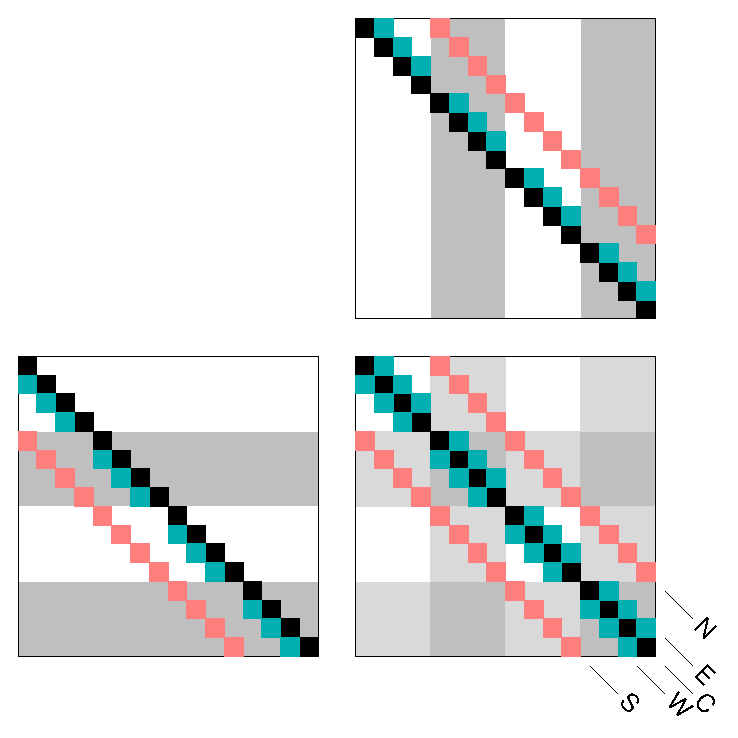
\includegraphics[height=6.0cm]{Incomplete_Cholesky_Compass.eps}}
  \end{picture}
\end{figure}

Diagonal entries of the L matrix ($b, s, w < i$):

\begin{eqnarray}
  l_{i,c} = \sqrt{a_{i,c} - a_{i,b}^2 - a_{i,s}^2 - a_{i,w}^2} \\
  l_{i,b} = a_{i,b} / l_{i,c}                                  \\
  l_{i,s} = a_{i,s} / l_{i,c}                                  \\
  l_{i,w} = a_{i,w} / l_{i,c}
\end{eqnarray}

Obviuousy, it is enough to store diagonal entries of the L matrix.

%==================================================%
%                                                  %
%   Solution of linear system with factorization   %
%                                                  %
%==================================================%
\section{Solution of linear system with factorization}

%======================%
%   LU decomposition   %
%======================%
\subsection{LU decomposition}

\begin{equation}
  \bf{A} \bf{x} = \bf{b}
\end{equation}

\begin{equation}
  \bf{A} = \bf{L} \bf{U}
\end{equation}

\begin{equation}
  \bf{L} \underbrace{\bf{U} \bf{x}}_y  = \bf{b}
\end{equation}

Forward solve:

\begin{equation}
  \bf{L} y  = \bf{b}
\end{equation}

Backward solve:

\begin{equation}
  \bf{U} x  = \bf{y}
\end{equation}

%============================%
%   Cholesky decomposition   %
%============================%
\subsection{Cholesky decomposition}

\begin{equation}
  \bf{A} \bf{x} = \bf{b}
\end{equation}

\begin{equation}
  \bf{A} = \bf{L} \bf{L}^T
\end{equation}

\begin{equation}
  \bf{L} \underbrace{\bf{L}^T \bf{x}}_y  = \bf{b}
\end{equation}

\subsubsection{Forward solve}

%-----------%
%  Forward  %
%-----------%
\begin{figure}[h!]
  \centering
  \setlength{\unitlength}{1mm}
  \begin{picture}(60,30)(0,0)
%-> \thicklines\put(0,0){\framebox(63,80){}}
    \put( 1,0){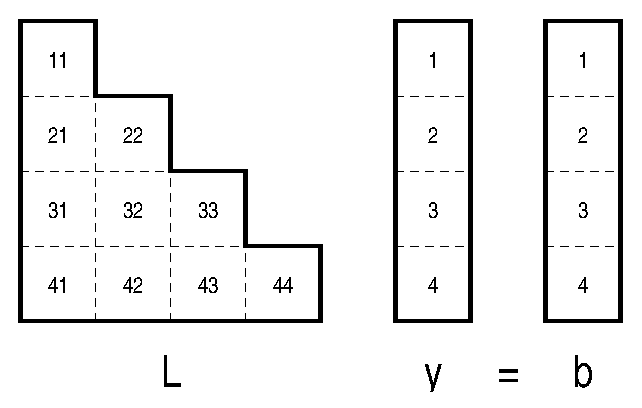
\includegraphics[height=3.0cm]{Forward.eps}}
  \end{picture}
\end{figure}

\begin{equation}
  \bf{L} y  = \bf{b}
\end{equation}

\begin{eqnarray}
  i & = & 1 \rightarrow N \\
  y_i  & = & (b_i - l_{b,i}y_{b,i} - l_{s,i}y_{s,i} - l_{w,i}y_{w,i}) / l_{c,i}
\end{eqnarray}

\subsubsection{Backward solve}

%------------%
%  Backward  %
%------------%
\begin{figure}[h!]
  \centering
  \setlength{\unitlength}{1mm}
  \begin{picture}(60,30)(0,0)
%-> \thicklines\put(0,0){\framebox(63,80){}}
    \put( 1,0){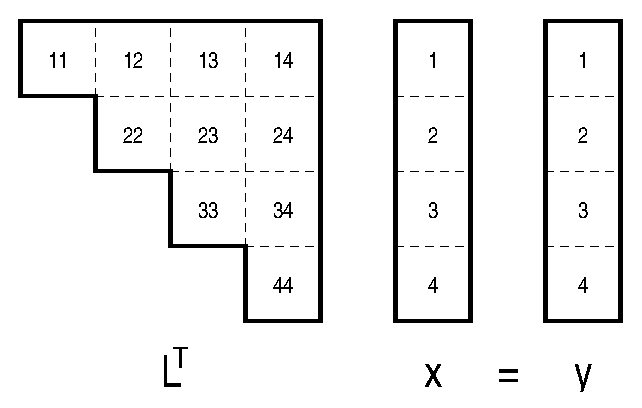
\includegraphics[height=3.0cm]{Backward.eps}}
  \end{picture}
\end{figure}

\begin{equation}
  \bf{L}^T x  = \bf{y}
\end{equation}

\begin{eqnarray}
  i & = & N \rightarrow 1 \\
  x_i  & = & (y_i - l_{t,i}x_{t,i} - l_{n,i}x_{n,i} - l_{e,i}x_{e,i}) / l_{c,i}
\end{eqnarray}

\end{document}
